\begin{figure*}[ht!]
    \centering
    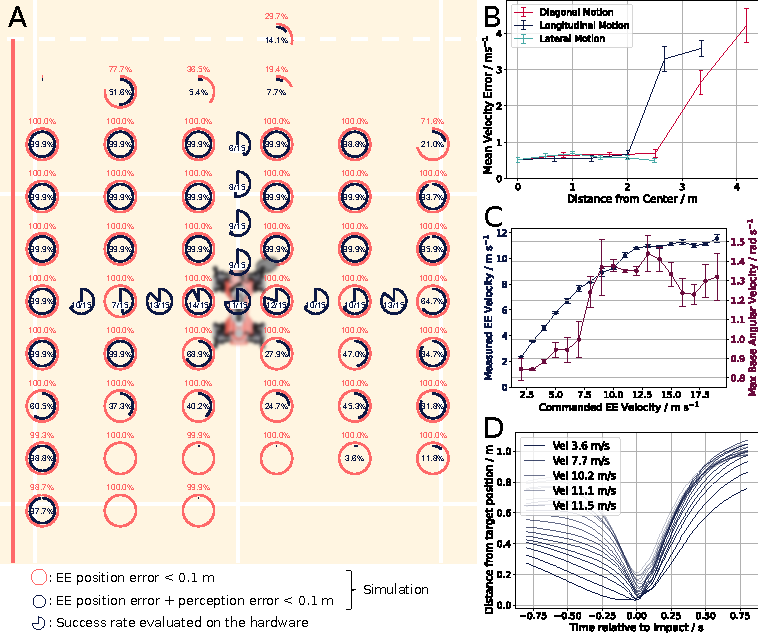
\includegraphics[width=0.9\textwidth]{Figures/SuccessRate/fig3_increased_font_size.pdf}
    \caption{\textbf{Assessing the controlled racket swings. (A)} We quantitatively evaluated the control system's success rate with progressively more difficult conditions in simulation and partly on the hardware. The EE position error condition evaluates the robot's ability to reach EE targets across the court; the additional perception error condition assesses the robot's ability to perform coordinated perception and control. On the hardware, we evaluated the robot's ability to hit the shuttlecock back across the net at intervals of \unit[0.5]{m}. The target and robot's initial positions are drawn to their corresponding position on the badminton court. \textbf{(B)} The EE velocity tracking error at interception increases as the robot attempts to hit shuttlecocks landing further from the court center. The error bars represent the standard deviation of the error across 6600 trials. \textbf{(C)} The EE swing velocity and maximum base angular velocity are plotted against the commanded EE velocity, with the error bar spanning from the minimum to maximum values. The robot is able to reach a maximum executed swing velocity of \unit[12.06]{ms$^{-1}$}, with generally increased base angular velocities at higher EE velocity commands.  \textbf{(D)} The distance between the racket sweet spot and the target impact position over relative time. The end-effector minimizes this distance precisely at the commanded impact time. The evaluations in \textbf{(C-D)} are conducted on the hardware.}
    \label{fig:success_rate}
    
    % \vspace{-1.5em}
\end{figure*}
